\section{BB84}
  \rhead{BB84}

  \subsection{Ohne Lauscher}
  Die Verschl\"usselte Kommunikation soll zwischen Alice und Bob stattfinden.
  F\"ur das BB84 Protokoll sind zwei Kommunikationskan\"ale n\"otig:
  Einen konventionellen, sowie ein optisches Medium.
  Alice beginnt polarisierte Photonen zu erstellen und \"uber das optische Medium an Bob zu senden.
  Dabei verwendet sie eine der zwei um $45^{\circ}$ verschobenen Basen,
  welche jeweils zwei um $90^{\circ}$ verschobene Polarisierungen aufweisen und damit die Werte 1 und 0 repr\"asentieren:

  \begin{tabular}{l l || c c}
    $(+)$ & rectilinear & $(\uparrow)$ & $(\rightarrow)$\\
    $(\times)$ & diagonal & $(\nearrow)$ & $(\searrow)$\\
    \hline
    & & $0$ & $1$\\
  \end{tabular}

  Die polarisierten Photonen dienen also als Qubits, das Quanten\"aquivalent eines konventionellen Bits.
  Dabei muss sich Alice die Reihenfolge der verwendeten Basen merken,
  denn sie werden sp\"ater ben\"otigt um eine statistische Analyse der \"Ubertragungsfehler zu erstellen.

  Bob nimmt die polarisierten Photonen entgegen und w\"ahlt zuf\"allig eine der beiden Basen aus durch welche er das Photon analysiert.
  Dabei w\"ahlt Bob mit $P(richtig)=0.5$ die richtige Basis.
  W\"ahlt Bob die falsche Basis erh\"alt er mit $P(korrekt|falsch)=0.5$ das korrekte Resultat,
  bei $P(korrekt|richtig)=1$ f\"ur das korrekte Resultat bei der richtigen Basis ergibt das ein $P(korrekt)=0.75$,
  dass ein Photon korrekt gemessen wurde.

  Nachdem gen\"ugend Photonen um ein ausreichend starken symmetrischen Schl\"ussel zu erzeugen gesendet wurden, findet zwischen Alice und Bob die sogenannte Basendiskussion statt.
  Dazu sendet Bob die Information, welche Basis er f\"ur welches Photon verwendete, \"uber den konventionellen Kanal zu Alice.
  Alice meldet ihm, bei bei welchen Photonen er die richtige Basis, also dieselbe, welche auch sie f\"ur die Polarisation verwandte, verwendet hat.
  Zur \"Uberpr\"ufung ob die Verbindung belauscht wurde f\"uhren Alice und Bob eine statistische Analyse der Verteilung der \"Ubertragungsfehler aus.
  Wenn die Verbindung nicht manipuliert wurde, ist mit $P(korrekt)=0.75$ zu rechnen.

  Beispiel:
  \begin{center}
    \begin{tabular}{ l || c | c | c | c | c | c | c | r }
      \hline
      A's Zufallsbits & 0 &  1 & 1 & 0 & 1 & 0 & 0 & 1 \\
      \hline
      A's Basen & $+$ & $+$ & $\times $ & $+$ & $\times $ & $\times $ & $\times $ & $+$ \\
      \hline
      A's Polarisation & $\uparrow$ & $\rightarrow$ & $\searrow$ & $\uparrow$ & $\searrow$ & $\nearrow$ & $\nearrow$ & $\rightarrow$ \\
      \hline
      B's Basen & $+$ & $\times $ & $\times $ & $\times $ & $+$ & $\times $ & $+$ & $+$ \\
      \hline
      B's Polarisation & $\uparrow$ & $\nearrow$ & $\searrow$ & $\nearrow$ & $\rightarrow$ & $\nearrow$ & $\rightarrow$ & $\rightarrow$ \\
      \hline
      B's gemessene Bits & 0 & 0 & 1 & 0 & 1 & 0 & 1 & 1 \\
      \hline
      Basen Diskussion \\
      \hline
      Shared Key Bits& 0 & & 1 & & & 0 & & 1 \\
      \hline
    \end{tabular}
  \end{center}

  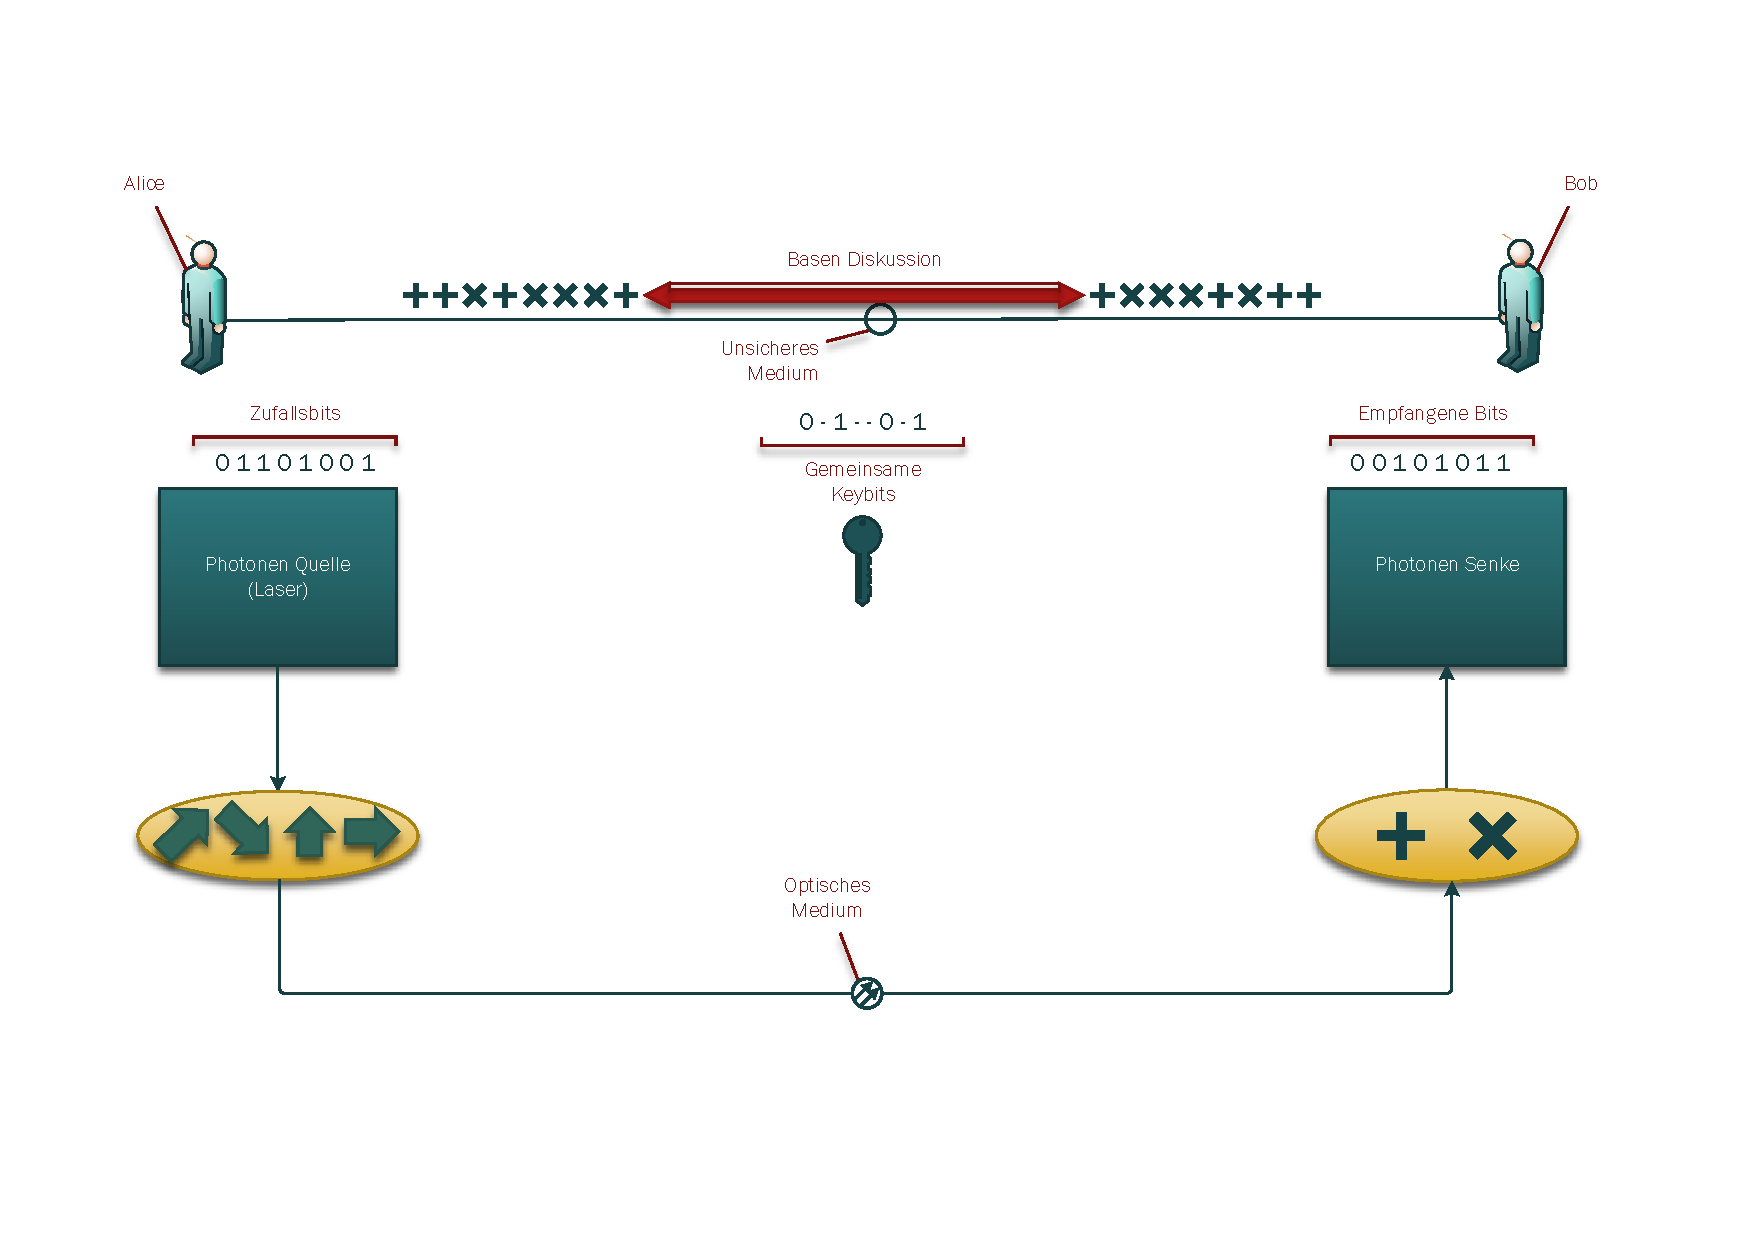
\includegraphics[width=\textwidth]{crypto/BB84.pdf}

  \subsection{Mit Lauscher}
  Das BB84 Protokoll erm\"oglicht es, einen Lauscher (Eavesdropper) zu bemerken.
  In konventionellen Schl\"usselaustausch Protokollen z.B.(DH, ECDH)
  beruht die Sicherheit des Schl\"ussels auf der mathematischen Komplexit\"at.
  Einem Lauscher ist es also m\"oglich den Schl\"ussel zu errechnen,
  wenn er nur einen ausreichend leistungsf\"ahigen Rechner hat.

  Beim BB84 Protokoll kann ein Lauscher jedoch nicht lauschen, ohne die \"Ubertragung zu beinflussen.
  Doch warum? Was \"andert sich wenn Eve lauscht?
  Eve f\"angt die von Alice polarisierten Photonen ab und misst sie mit 50\% Wahrscheinlichkeit korrekt.
  $P(\times)=0.5, P(+)=0.5$
  Danach generiert Eve ein neues Photon, mit derselben Polarisation,
  wie die, welche sie gemessen hat und sendet es weiter zu Bob.
  Da Eve auch nur mit $P(korrekt)=0.75$ korrekt misst, kann sie auch nur in $75^{\circ}$ der F\"alle die richtige Polarisation erzeugen.
  Bob kann also nur noch mit $P(korrekt|Eve-korrekt)=0.75*0.75=0.625$ die korrekte Polarisation messen.
  Um dies festzustellen tauschen Alice und Bob einige Schl\"usselbits aus,
  dazu werden sogenannte Decoypulses eingebaut, das sind Bits,
  welche nur f\"ur die Statistik dienen und nicht im Schl\"ussel verwendung finden.

  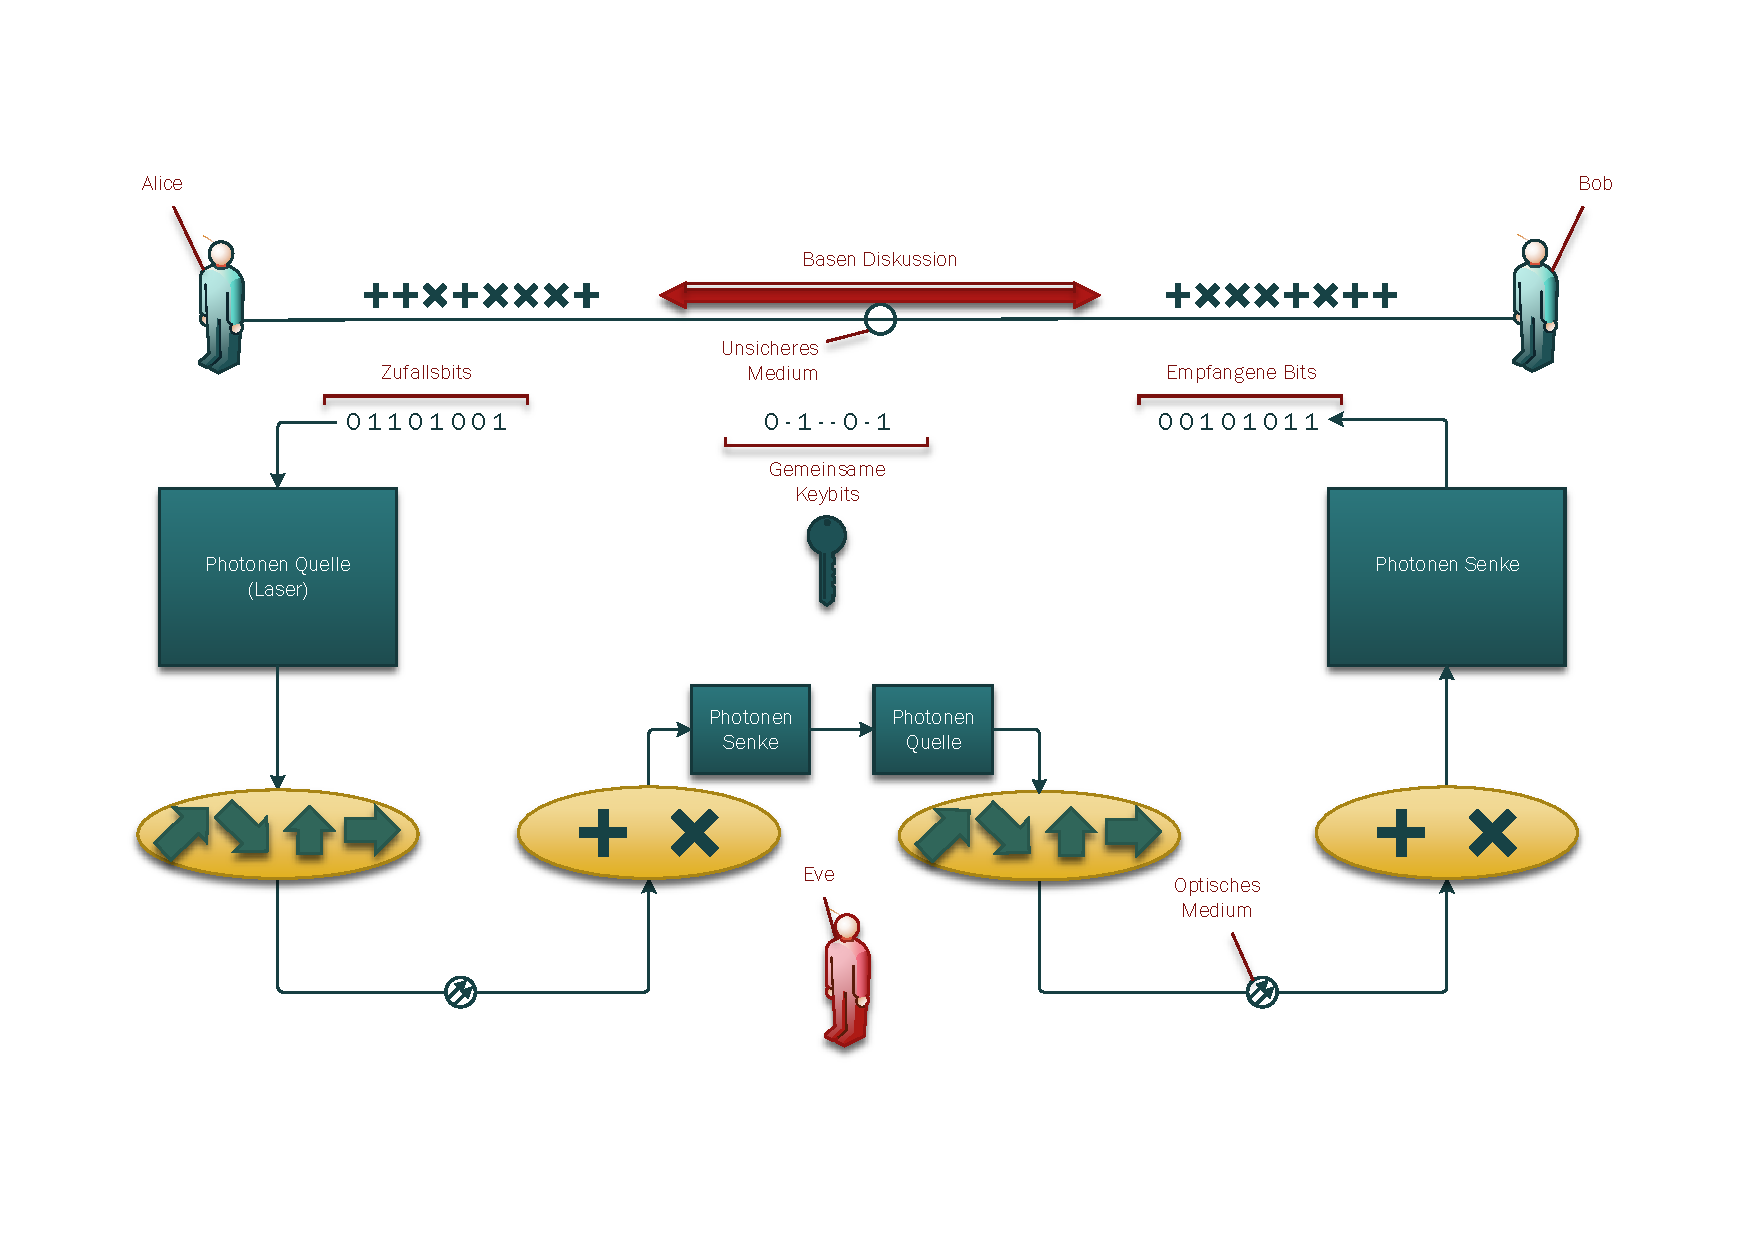
\includegraphics[width=\textwidth]{crypto/BB84Eve.pdf}

  Die einzige m\"ogliche Art von Eavesdropping ist, wenn Eve bei der Quelle die M\"oglichkeit hat, \"uberz\"ahlige Photonen abzuzweigen, sie zu lagern und nachdem Alice und Bob die Basendiskussion gef\"uhrt haben, mit dem der richtigen Basis zu messen und dadurch einzelne g\"ultige Keybits zu erhalten.

  \subsection{No-Cloning}
  Die Grundlage f\"ur das Funktionieren dieser Methode bietet die Tatsache, dass man nicht beliebige Zust\"ande auf einen anderen kopieren kann. Siehe No-Cloning-Theorem (NCT) \ref{skript:no-cloning-theorem}.
  Eve kann aufgrund des No-Cloning-Theorems die Photonen von Alice nicht einfach kopieren und die Kopie an Bob schicken,
  sondern ist gezwungen anhand ihrer Messungen (von denen h\"ochstens 75\% korrekt sind) selbst Photonen zu polarisieren
  und Bob zu senden, was bei Bob zu einer Trefferrate von weniger als 0.75 f\"uhrt.
  $P(korrekt|Eavesdropper)<0.75$
  Wenn man also Eve mit $P=0.999999999$ aufsp\"uren will,
  folgt aus dieser Formel $P_d = 1 - \left(\frac{3}{4}\right)^n$,
  dass 72 Keybits ausgetauscht werden m\"ussen.

  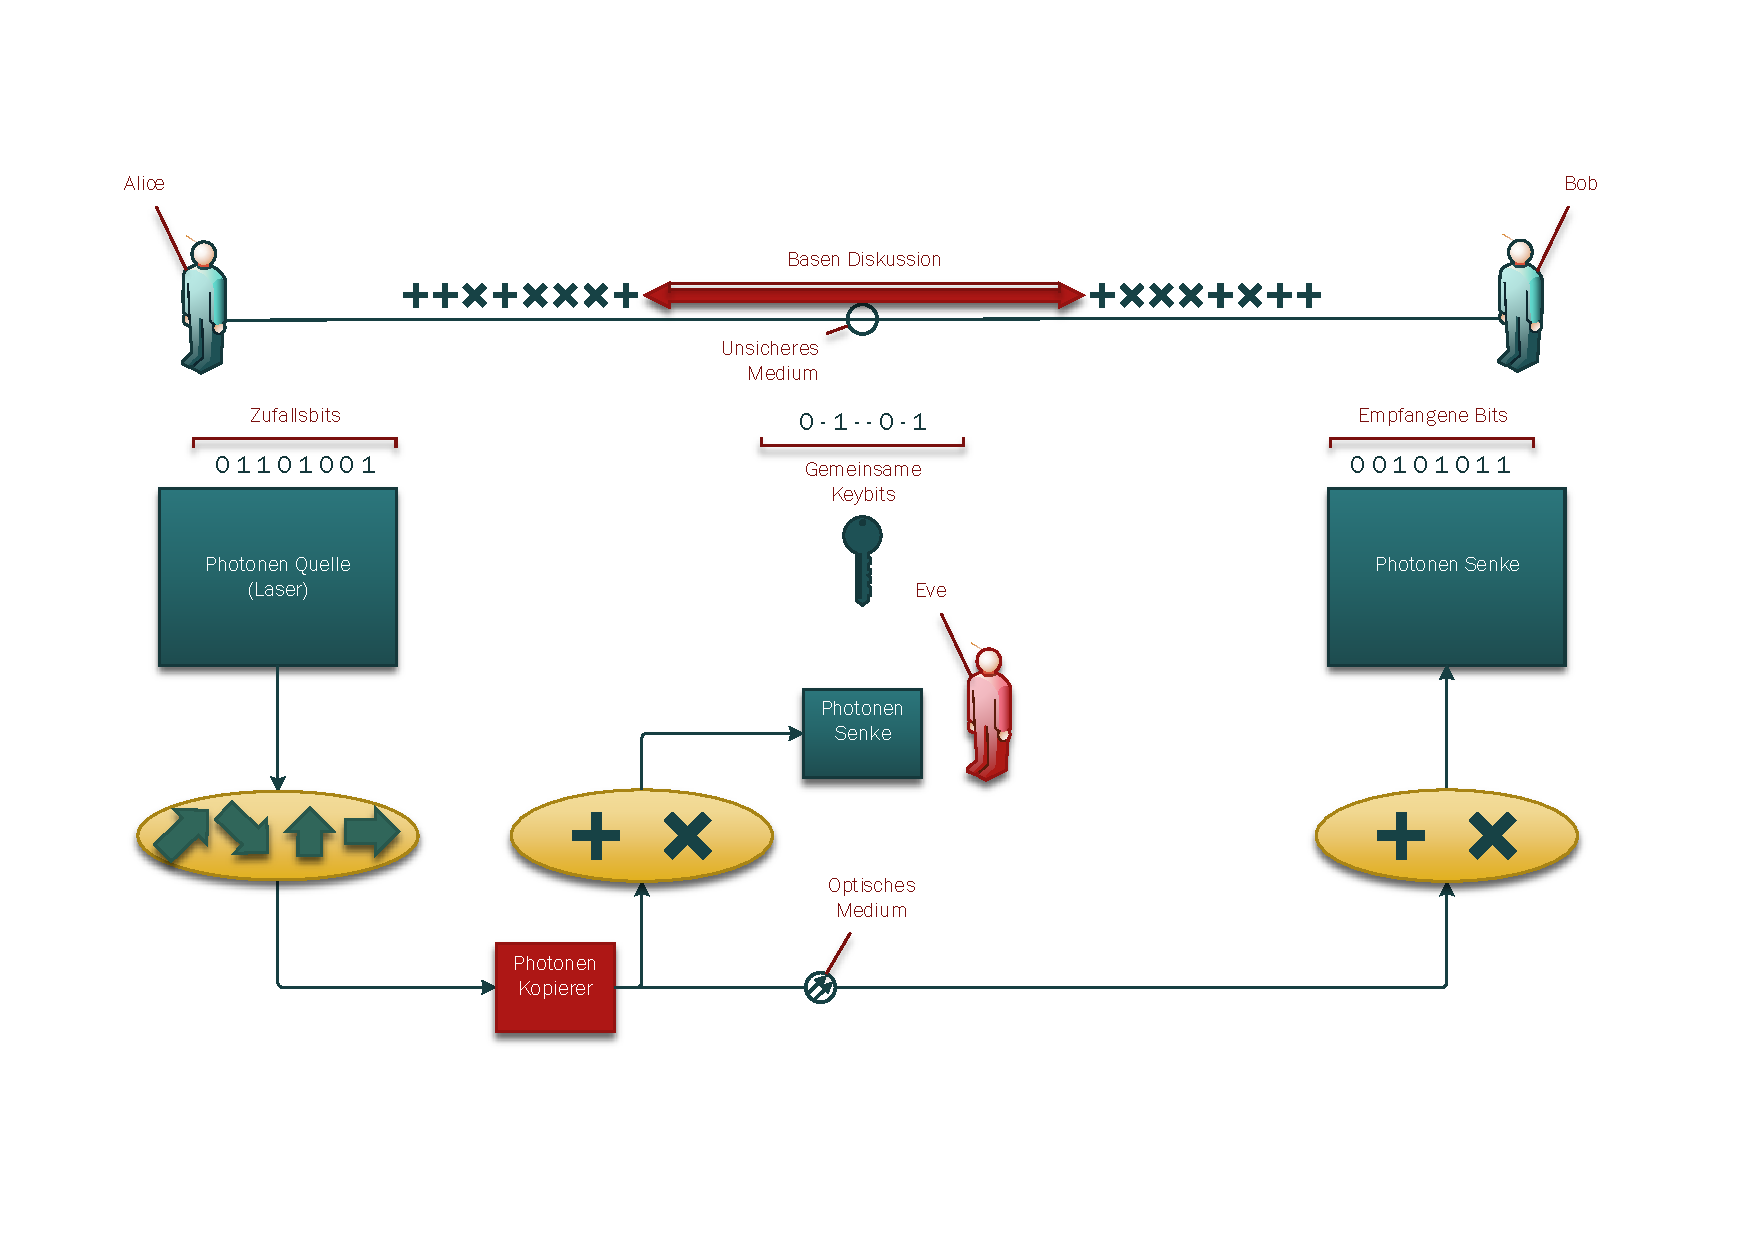
\includegraphics[width=\textwidth]{crypto/BB84Eve-Clone.pdf}

  \subsection{Mit Man-In-The-Middle}
  Das BB84 Protokoll sch\"utzt jedoch nicht vor einer MitM Attacke,
  jedoch kann dazu eine Authentisierung des Partners verwendet werden.\cite{qc:Authentisierung}

  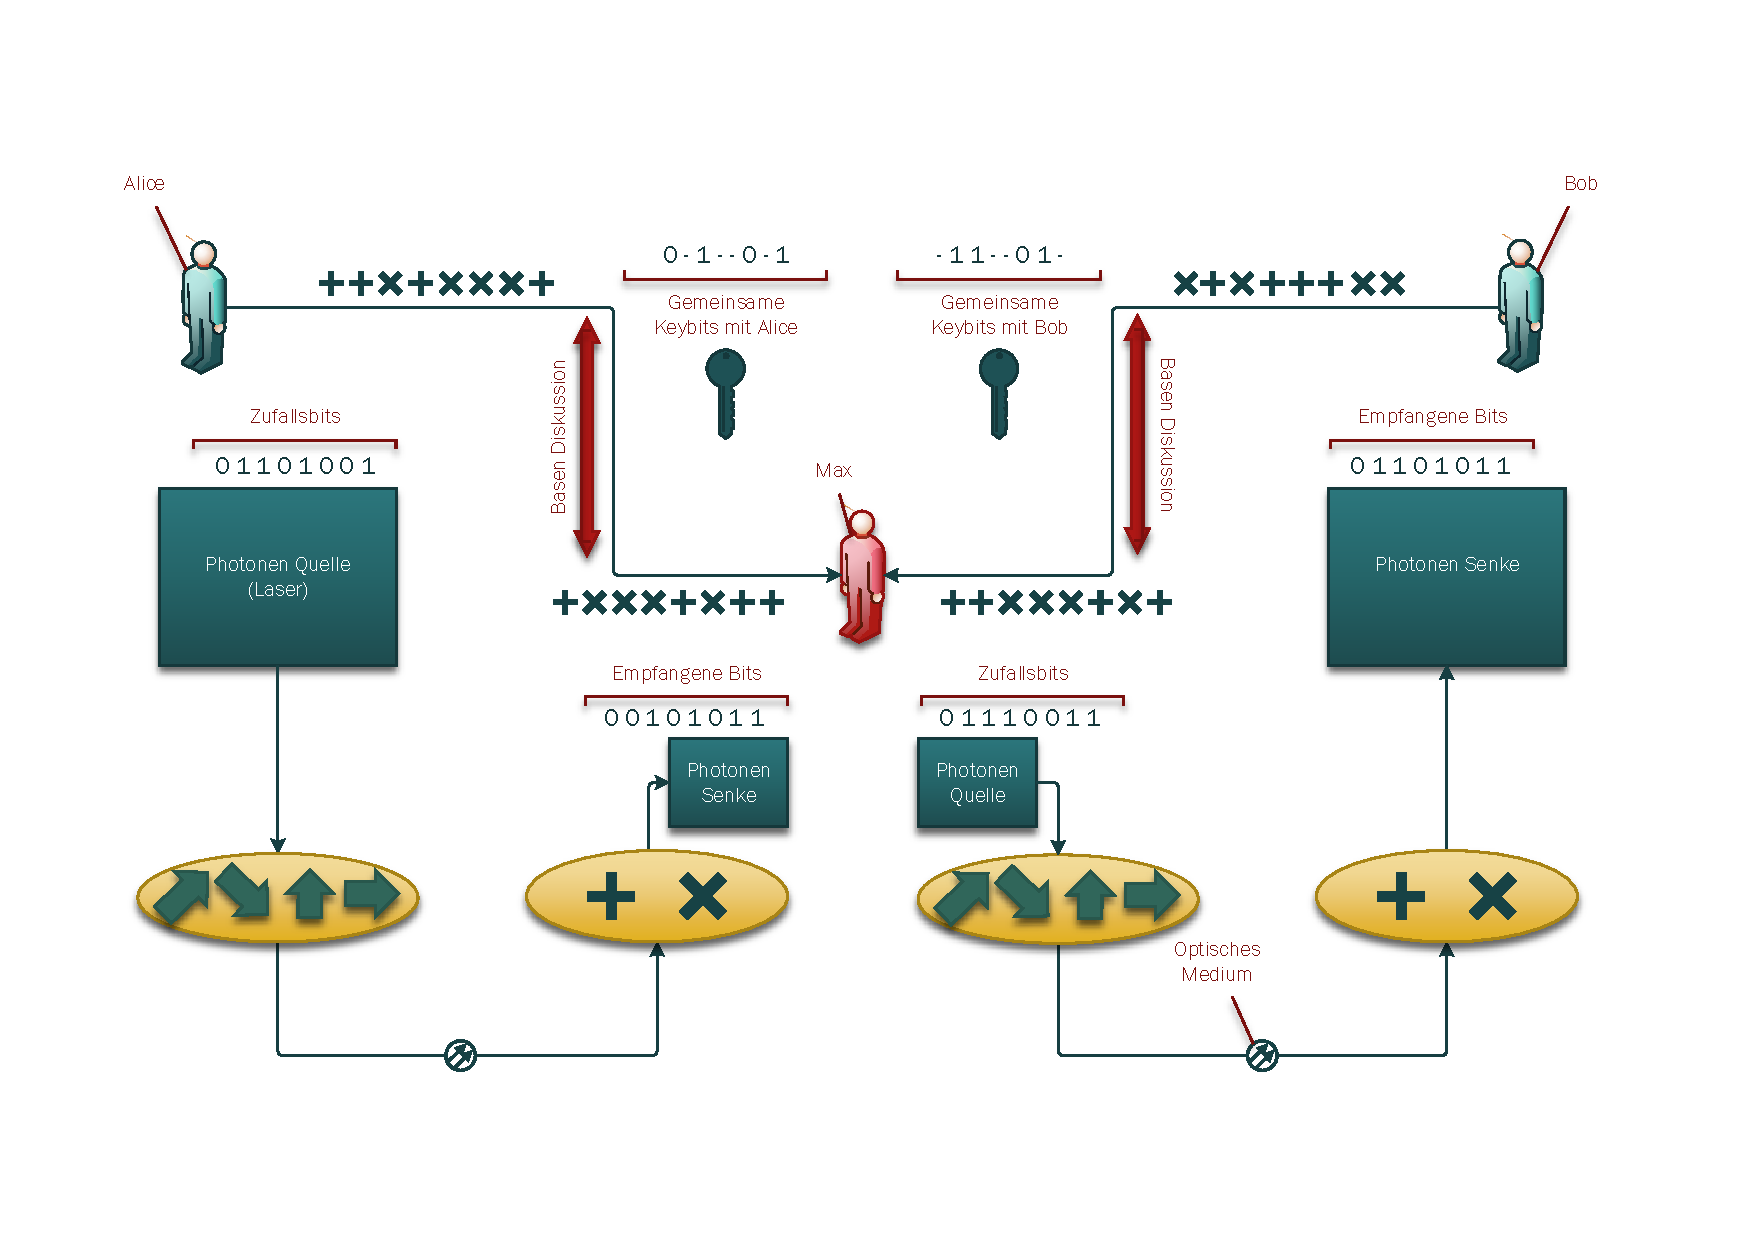
\includegraphics[width=\textwidth]{crypto/BB84Max.pdf}

